\chapter{Experiments and Analysis}
\label{ch:result}

    We have divided the experiments into two parts. In the first part, We analyze the protocol under different scenarios. In the latter part, we compare the performance of the HoneyBadgerBFT with Raft as ordering service in Hyperledger Fabric.
    \section{Protocol Performance}
    In this section, we test the protocol performance under different network scenarios, different workloads, and analyze it.
    \subsection{Unstable Network}
    In the section, the protocol is tested when the underlying network is not stable, and the network fluctuates from time to time. We found out that the protocol makes progress whenever the network is running and closely replicates the network performance.
    \\\\
   \textbf{Test setup :}\\
  %%TODO update table
\begin{table}[!h]
\centering
\begin{tabular}{ |r|  l| }
\hline
 \textbf{Machine}&  \\
 \hline
  OS & Ubuntu 18.02 \\  
   CPU & Intel Xeon v2 processor 2 cores \\
  Memory &8 GB\\
  \hline
  \textbf{Nodes}&\\
  \hline
Nodes  &4 \\
Machines & 4\\
\hline
\textbf{Protocol Parameters}&\\
\hline
Input TPS & 30 transactions\\
Batch Size & 30 transactions\\
  \hline
\end{tabular}
\caption{Cluster node configurations for unstable network}
\end{table}

\begin{figure}[!h]
    \centering
    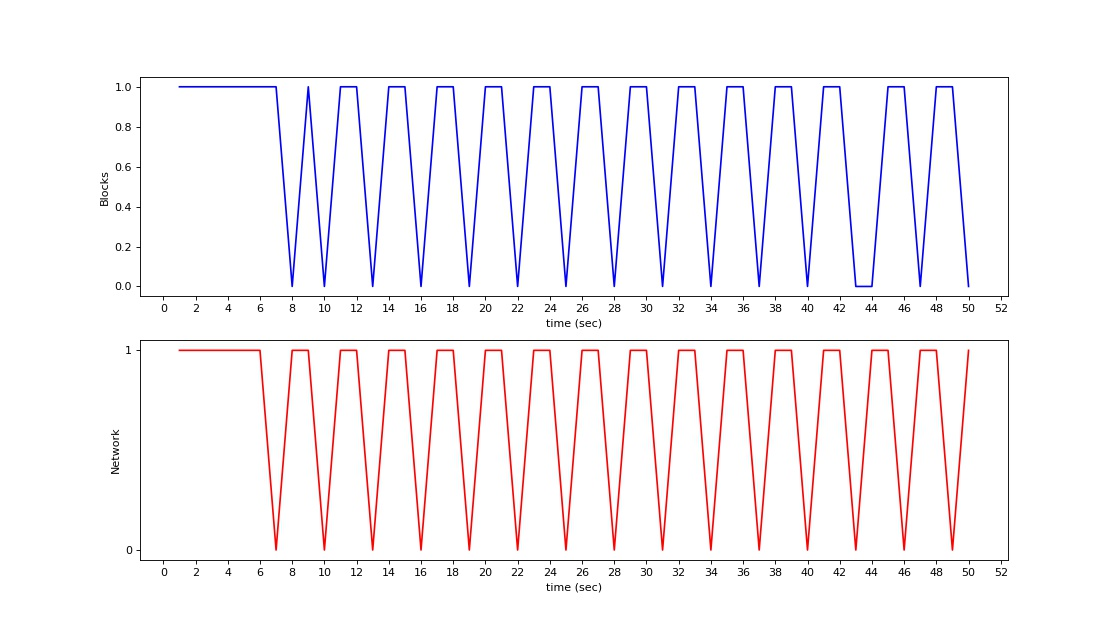
\includegraphics[width=1\textwidth]{images/1_2.jpg}
    \caption{Every 2 second network is out for 1 sec}
    \label{fig:1_2}
\end{figure}
\begin{figure}[!h]
    \centering
    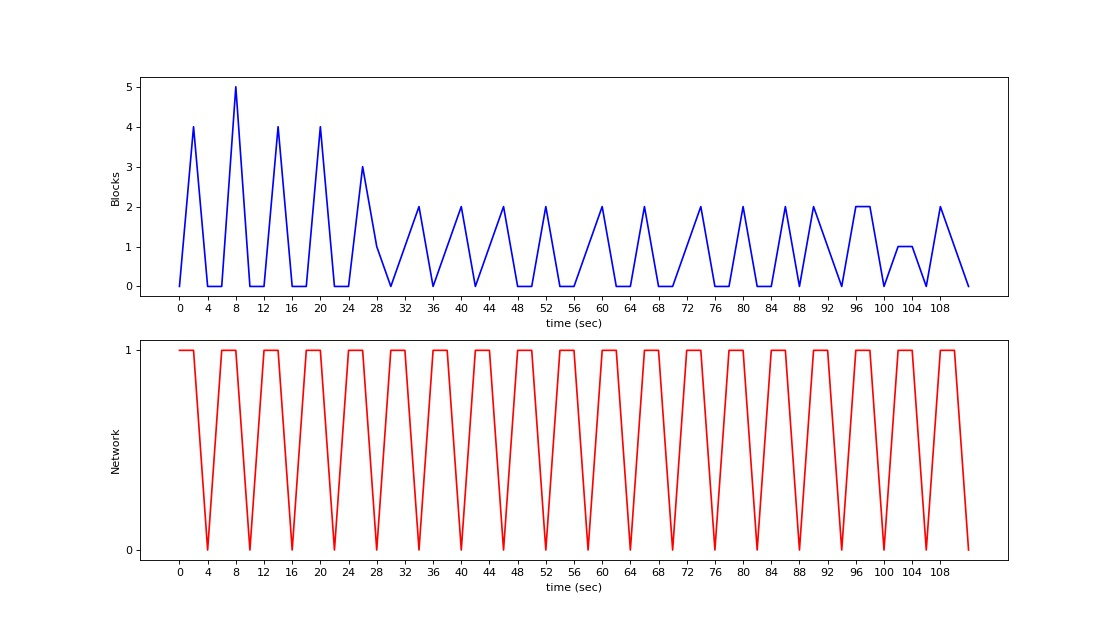
\includegraphics[width=1\textwidth]{images/2_4.jpg}
    \caption{Every 4 second network is out for 2 sec}
    \label{fig:2_4}
\end{figure}
\begin{figure}[!h]
    \centering
    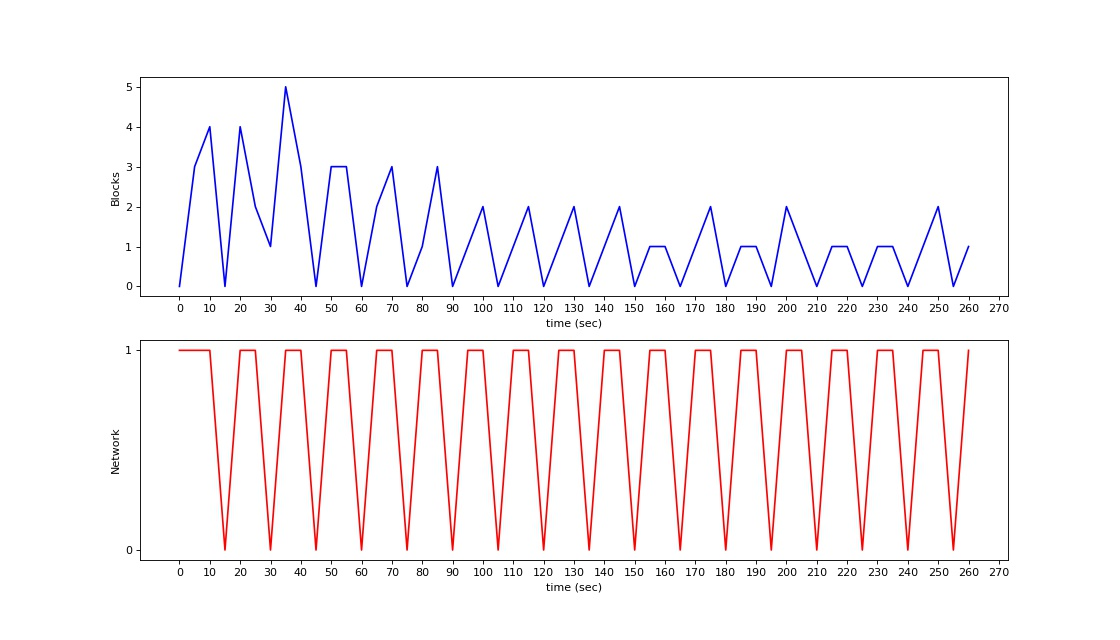
\includegraphics[width=1\textwidth]{images/5_10.jpg}
    \caption{Every 10 second network is out for 5 sec}
    \label{fig:5_10}
\end{figure}
\begin{figure}[!h]
    \centering
    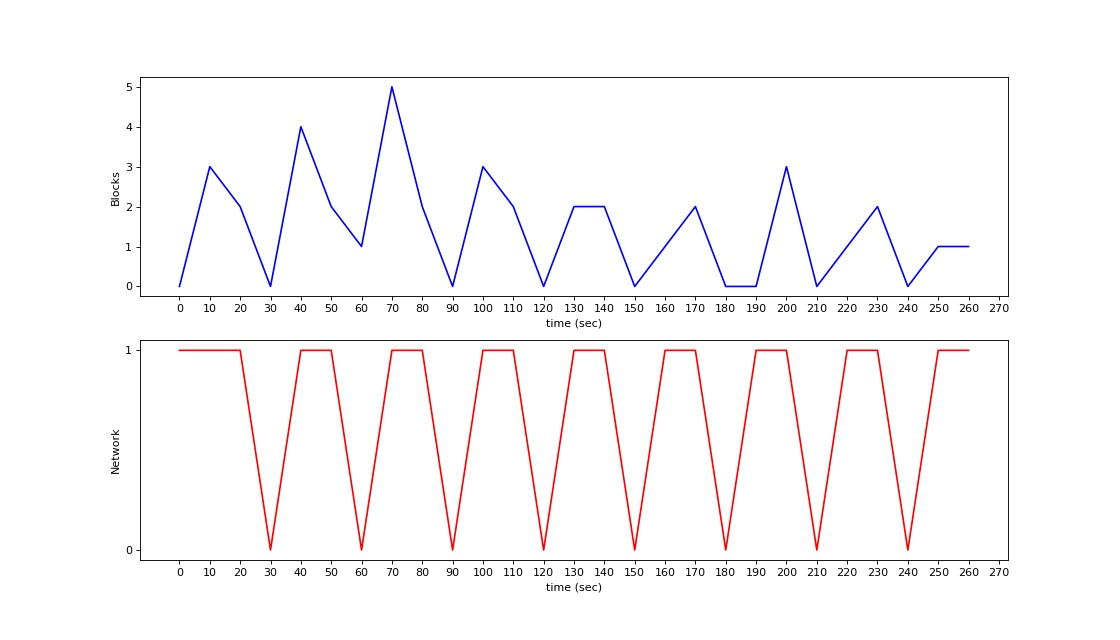
\includegraphics[width=1\textwidth]{images/10_20.jpg}
    \caption{Every 20 second network is out for 10 sec}
    \label{fig:10_20}
\end{figure}
\begin{figure}[!h]
    \centering
    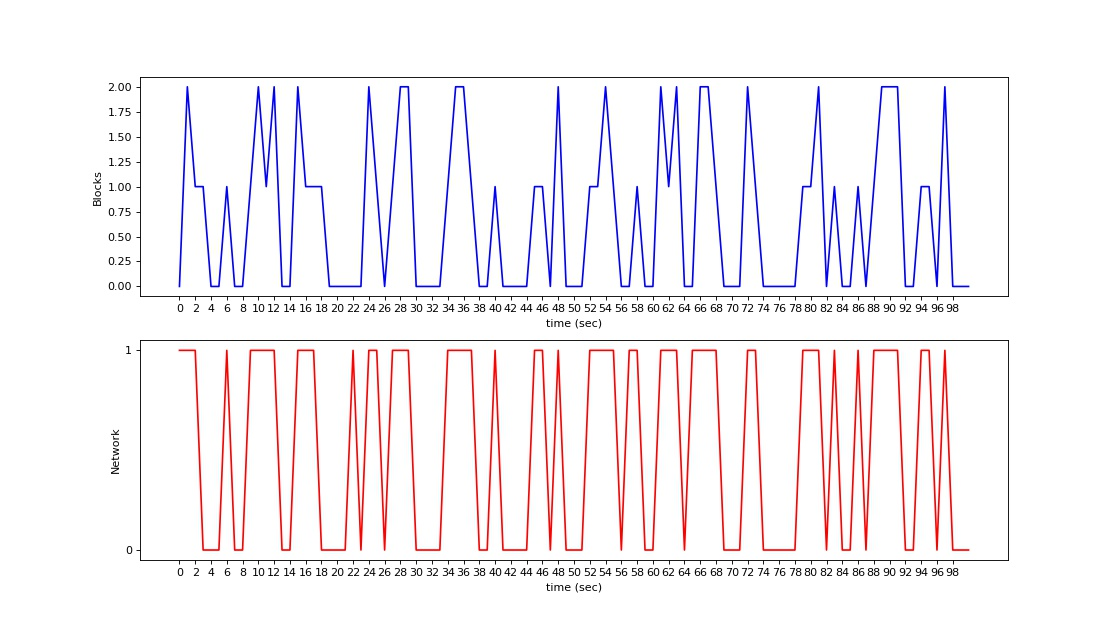
\includegraphics[width=1\textwidth]{images/5_random.jpg}
    \caption{Network is out for random time(maxed at 5 sec) after random seconds}
    \label{fig:5_random}
\end{figure}
\begin{figure}[!h]
    \centering
    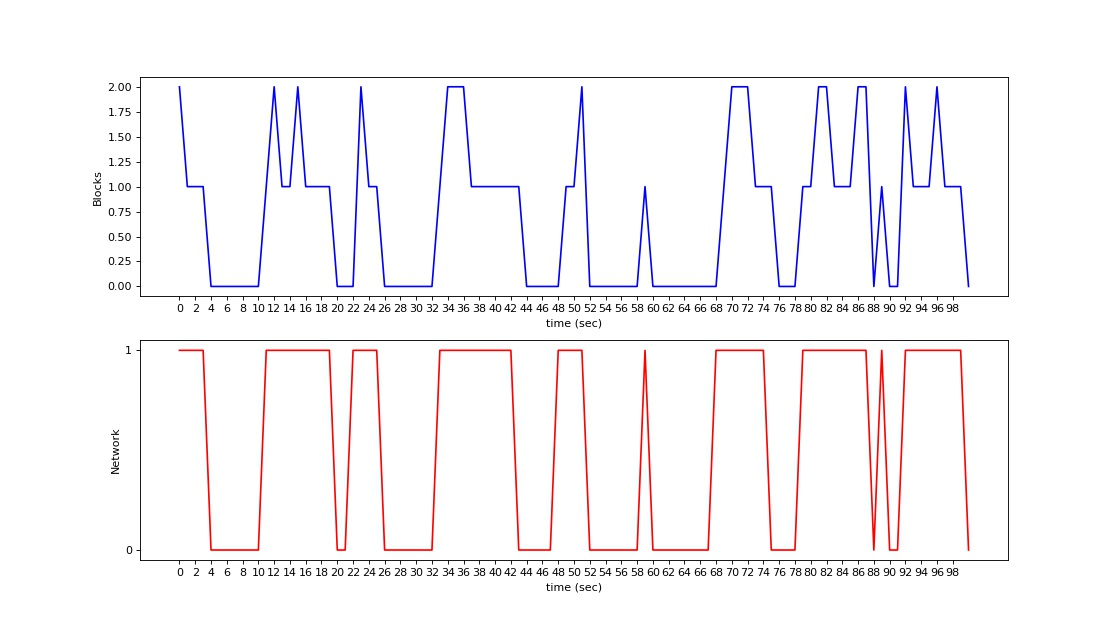
\includegraphics[width=1\textwidth]{images/10_random.jpg}
    \caption{Network is out for random time(maxed at 10 sec) after random seconds}
    \label{fig:10_random}
\end{figure}
\clearpage
In above figures, the plot in blue show number of blocks committed in that period of time. The plot in red shows the condition of the network in that period where `1' indicates that network is up and `0' indicates network is down.

In Figures \ref{fig:1_2}, \ref{fig:2_4}, \ref{fig:5_10} and \ref{fig:10_20}, The network is down for a certain fixed period of time and then up for a certain fixed period of time alternatively. For example, In figure \ref{fig:1_2}, the network is up for 2 seconds and then down for 1 second and then again up for 2 sec, and this goes on. Similarly, for other figures with different units of time. In figure \ref{fig:5_random} and \ref{fig:10_random} Network is behaving randomly. It goes down for a random period and then up for a random period.
In figure \ref{fig:5_random} max period is limited by 5 sec and in figure \ref{fig:10_random} max period is limited by 10 second.

To achieve this behaviour, we made the thread handling the network to go to sleep which simulates as the network is down as the thread is sleeping in that period no request of send or receive any network packet is processed.

\subsubsection{Analysis}
We can see from the above figures that the protocol is performing as expected. It is making progress as soon as the network is up, and its throughput is closely replicating the network performance no matter how bad and unpredictable the behaviour of the network is.
\subsection{Different Load Conditions and Different Cluster Setups}
In this section, we have tested the protocol over the network with different transaction sizes and block sizes to check the protocol's efficiency.

 \textbf{Test setup :}\\
   \begin{table}[!h]
   \centering
\begin{tabular}{ |r|  l| }
\hline
 \textbf{Machine} & \\
 \hline
  OS & Ubuntu 18.02 \\  
   CPU &Intel Xeon v2 processor 2 cores \\
  Memory &8 GB\\
  \hline
  \textbf{Nodes}&\\
  \hline
Nodes  &4\\
Machines & 4\\
\hline

\end{tabular}
\caption{Cluster node configurations for load testing}

\end{table}
% \subsubsection{4 nodes:}
\begin{figure}[!h]
    \centering
    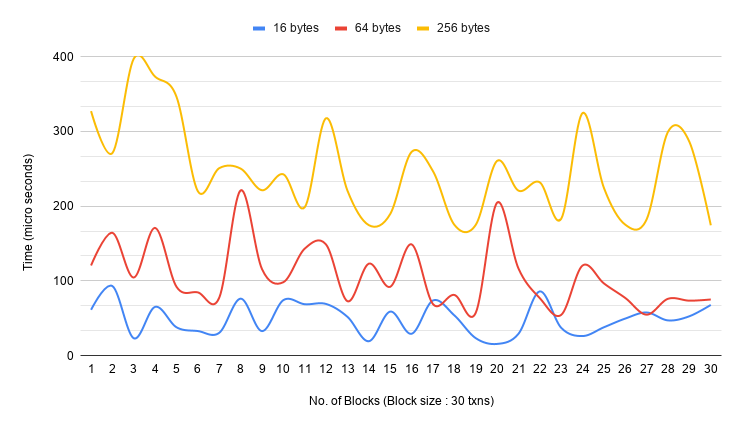
\includegraphics[scale=0.5]{images/4_nodes.png}
    \caption{Latency plot for different transaction sizes }
    \label{fig:4_nodes}
\end{figure}


% \subsubsection{8 nodes:}
\begin{figure}[!h]
    \centering
    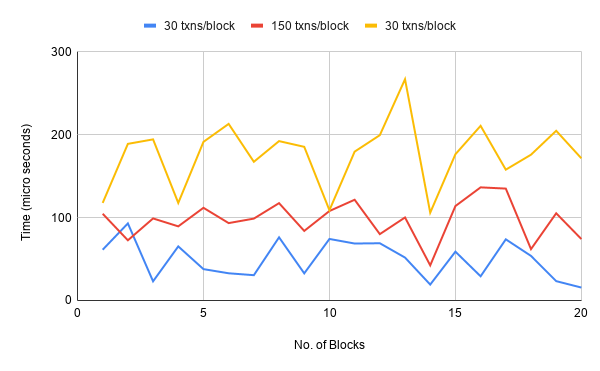
\includegraphics[scale=0.6]{images/4_block_size.png}
    \caption{Latency plot for different block sizes}
    \label{fig:4_batchsize}
\end{figure}
\clearpage
% \begin{figure}[!h]
%     \centering
%     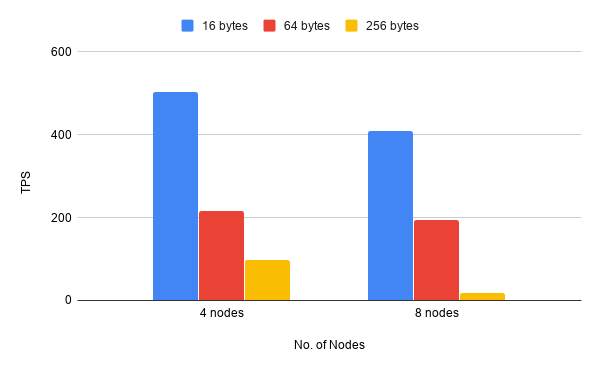
\includegraphics[scale=0.6]{images/4_8_tps.png}
%     \caption{TPS comparison between 4 nodes and 8 nodes}
%     \label{fig:4_8_tps}
% \end{figure}
% \subsubsection{Analysis}
\begin{figure}
\centering
\begin{subfigure}{.5\textwidth}
  \centering
  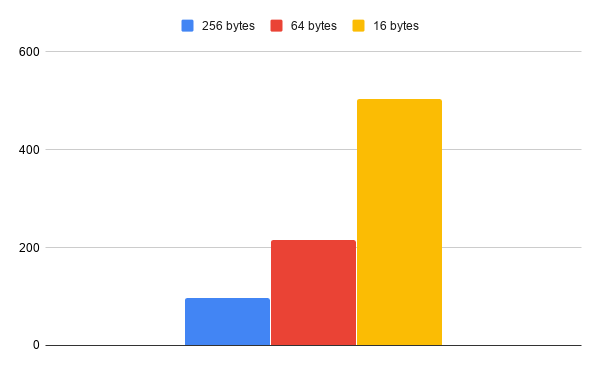
\includegraphics[width=1\linewidth]{images/tps_txnsize.png}
  \caption{Different Transaction Sizes}
  \label{fig:diff_txns}
\end{subfigure}%
\begin{subfigure}{.5\textwidth}
  \centering
  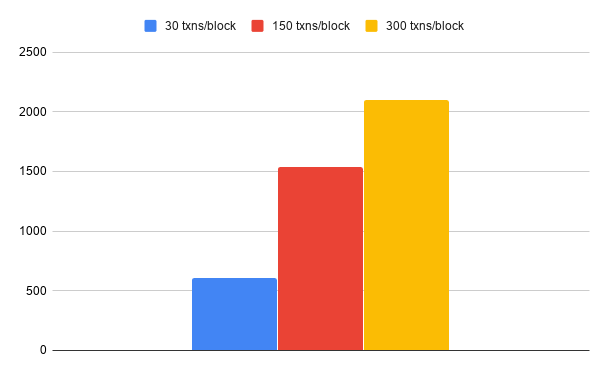
\includegraphics[width=1\linewidth]{images/tps_blocksize.png}
  \caption{Different Block Sizes}
  \label{fig:diff_batch}
\end{subfigure}
\caption{Throughput}
\label{fig:test}
\end{figure}
\subsubsection{Analysis}
We can see in figure \ref{fig:diff_txns} as the size of transaction decrease the throughput increase which shows that HoneyBadgerBFT’s throughput always closely tracks the network’s available bandwidth.

In Figure \ref{fig:diff_batch} and \ref{fig:4_batchsize} we see that we can achieve greater TPS if we can trade off on latency, As the batch size increase both latency and throughput increases.
User can choose between the low latency or high throughput. We were able to achieve a throughput of 2100 transactions/sec.




\section{HoneyBadgerBFT vs Raft}
In this section, We benchmark the performance of HoneyBadgerBFT vs. the performance of Raft under different conditions such as the different number of orderer nodes, different transaction rates, and the varied number of total transactions and compare their performances.

We used Hyperledger Caliper \cite{caliper_doc}\cite{caliper_white_paper} for the benchmarking. 
  \begin{table}[!h]
  \centering
\begin{tabular}{ |r|  l |}
\hline
 \textbf{Machine} & \\
 \hline
  OS & Ubuntu 18.02 \\  
   CPU & Intel Xeon v2 processor 2 cores \\
  Memory &8 GB\\
  \hline
  \textbf{Nodes}&\\
  \hline
Nodes  &4, 8 and 16\\
Machines & 4\\
\hline
\textbf{Protocol Parameters} & \\
\hline
Input TPS & 100, 40 ,30 transactions\\
Batch Size & 200 transactions\\
Batch Timeout & 2 sec\\
Total Transactions& 100, 1000 and 5000\\
  \hline
\end{tabular}
\caption{Cluster node configurations for Fabric network}

\end{table}
\clearpage
\subsection{Fabric Network Configuration}
We have used three cluster sizes i.e., 4 nodes, 8 nodes, and 16 nodes and tested all of them with three different combinations of total number of transactions and transaction rate i.e., transaction per second (tps). The combinations are a total of 100 transactions at 100 tps, 1000 transactions at 40 tps, and 5000 transactions at 30 tps. The performances of both Raft and HoneyBadgerBFT are shown in the plots below.
% \subsubsection{Raft}
\begin{figure}[!h]
    \centering
    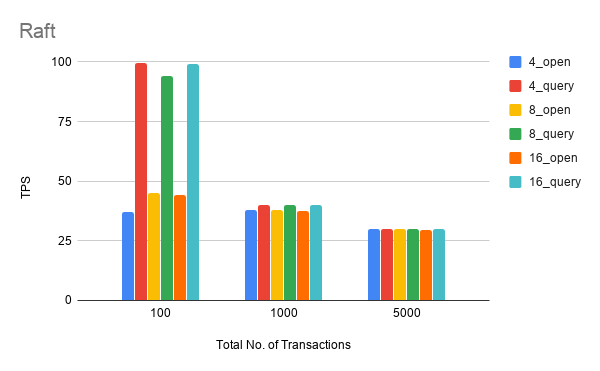
\includegraphics[scale=0.7]{images/raft_tps.png}
    \caption{Raft's Throughput}
    \label{fig:raft_tps}
\end{figure}
% \subsubsection{HoneyBadgerBFT}
\begin{figure}[!h]
    \centering
    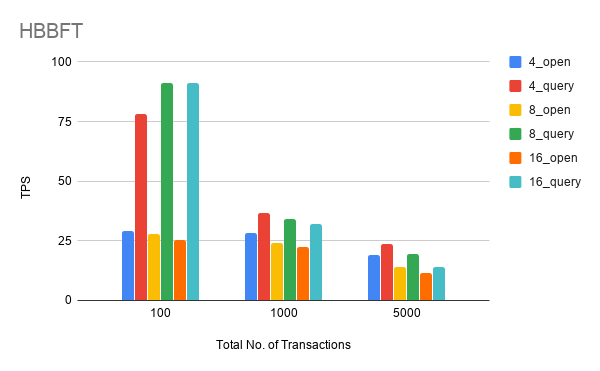
\includegraphics[scale=0.7]{images/hbbft_tps.png}
    \caption{HoneyBadgerBFT's Throughput}
    \label{fig:hbbft_tps}
\end{figure}
  
   \clearpage
   
 \begin{table}[!h]
 \centering
\begin{tabular}{ |C{1cm}|c|c|C{3cm}|c|}
\hline
 \textbf{No of Nodes} & \textbf{Orderer} & \textbf{Avg. Latency} & \textbf{Avg. CPU(max.) usages} & \textbf{Avg. RAM usages}  \\
 \hline
  \textbf{4} & Raft&1.72&    6.40&    15.23\\
  
  & HoneyBadgerBFT &3.43&    8.24&    46.4\\
  \hline
  \textbf{8} & Raft & 1.61&    3.99    &29.05\\
  
  & HoneyBadgerBFT &5.42&    8.13&    44.3\\
  \hline
  \textbf{16} & Raft&1.76&    2.33&    32.06\\
  
  & HoneyBadgerBFT &8.26    &12.13&    88.67\\
  
  \hline
  
\end{tabular}
\caption{Comparison with Raft}

\end{table}

\subsubsection{Analysis}
From the benchmark results, we found that the throughput of HoneyBadgerBFT is less than Raft, but it is acceptable as HoneyBadgerBFT is Byzantine Fault Tolerant, whereas Raft is only Crash Fault Tolerant. But throughput is comparable and is not significantly low.

We achieve much higher throughput than Elastico, which is also BFT protocol implementated by Ayushi Aggarwal in her Master's thesis, in 2019 \cite{elastico}. Elastico achieves 0.5 tps, whereas HoneybadgerBFT achieves 29 tps, which is a gain of 580\%.

Resource utilization is slightly higher than the Raft, which is also acceptable given Raft is only CFT.


Overall, HoneyBadgerBFT performs well as ordering service in Fabric and can be used in the real-world application as an alternative to Raft as it provides Byzantine Fault Tolerance with a small hit on performance with an added benefit that it can work in any network conditions.
